% Scheme of the three-layer model of cognitive tasks involved while driving.
% The figure illustrates the Hierarchical Control Model proposed by Michon.
%
\documentclass{standalone}
\usepackage{tikz}

\begin{document}
	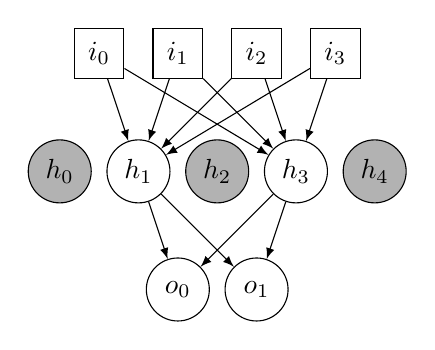
\begin{tikzpicture}[
			ci/.style={draw, circle, minimum size=8mm},
			dci/.style={draw, circle, minimum size=8mm, fill=black!30},
			sq/.style={draw, inner sep=5}
		]
		\node[sq] at (-1.5,0) (i0) {$i_0$};
		\node[sq] at (-0.5,0) (i1) {$i_1$};
		\node[sq] at (0.5,0) (i2) {$i_2$};
		\node[sq] at (1.5,0) (i3) {$i_3$};			
		\node[dci] at (-2,-1.5) (h0) {$h_0$};
		\node[ci] at (-1,-1.5) (h1) {$h_1$};
		\node[dci] at (0,-1.5) (h2) {$h_2$};
		\node[ci] at (1,-1.5) (h3) {$h_3$};			
		\node[dci] at (2,-1.5) (h4) {$h_4$};			
		\node[ci] at (-0.5,-3) (o0) {$o_0$};			
		\node[ci] at (0.5,-3) (o1) {$o_1$};			
		
		\foreach \a in {0, 1, 2, 3}{
			\foreach \b in {1, 3}
			\draw[-latex] (i\a) -- (h\b);
		}
		\foreach \a in {1, 3}{
			\foreach \b in {0, 1}
			\draw[-latex] (h\a) -- (o\b);
		}
		
	\end{tikzpicture}
\end{document}